%% SoftwareX Original Software Publication — dirac_wavepacket
%% Based on the official OSP LaTeX template (v2026).
%% Target: ~3500 words main text, 5 figures, 6 pages.
%%
%% NOTE ON PACKAGE NAME: the package is still referred to as "dirac_wavepacket"
%% throughout. Before final submission, search-and-replace with the final
%% chosen name (candidate list in repo: tiltwave, valleyflow, dtrans2d,
%% wavepacket2d, klein2d, spinorflow, borotrans, cone2d).

\documentclass[preprint, 12pt, a4paper]{elsarticle}

\usepackage{amssymb}
\usepackage{amsmath}
\usepackage{hyperref}
\usepackage{booktabs}
\usepackage{xspace}
\setlength{\parindent}{0pt}
\setlength{\parskip}{0.6em plus 0.1em minus 0.1em}

\newcommand{\dirac}{\texttt{dirac\_wavepacket}\xspace}
\newcommand{\vF}{v_\mathrm{F}}
\newcommand{\EF}{E_\mathrm{F}}

\journal{SoftwareX}

\begin{document}
\renewcommand{\labelenumii}{\arabic{enumi}.\arabic{enumii}}

\begin{frontmatter}

\title{\texttt{dirac\_wavepacket}: wave-packet transport in two-dimensional tilted
       Dirac and Weyl systems}

\author[nrc]{Can Yesilyurt\corref{cor}}
\ead{cyesil@nanorescenter.com}

\cortext[cor]{Corresponding author.}

\address[nrc]{Nanoelectronics Research Center, Istanbul, Turkey}

\begin{abstract}
\dirac is an open-source Python package for time-dependent transport
of wave packets in two-dimensional Dirac and Weyl systems with
anisotropic Fermi velocities and tilted cones. A two-component spinor
is evolved on a uniform grid by a second-order symmetric
split-operator Fourier scheme whose momentum step is an analytical
$2\times2$ unitary. Arbitrary polygonal or rotated barrier
geometries, absorbing drain contacts that double as transmission and
reflection detectors, mass-confined reflecting walls, and an
optional $4$-component coupled propagator for intervalley coupling
are supported together in a single workflow. The code is installed
via \texttt{pip}, validated by a pytest suite, and released under
the MIT licence.
\end{abstract}

\begin{keyword}
Dirac equation \sep Weyl semimetal \sep tilted cone \sep valley
transport \sep split-operator FFT \sep wave-packet dynamics
\end{keyword}

\end{frontmatter}

% =======================================================================
\section*{Required Metadata}
\label{}

\section*{Current code version}
\label{}

\begin{table}[!h]
\small
\begin{tabular}{|c|p{4.8cm}|p{6.8cm}|}
\hline
\textbf{Nr.} & \textbf{Code metadata description} & \textbf{Value} \\
\hline
C1 & Current code version & v1.0.0 \\
\hline
C2 & Permanent GitHub link to code/repository used for this code version &
    \href{https://github.com/can-yesilyurt/Dirac-Wavepacket}%
         {\nolinkurl{github.com/can-yesilyurt/Dirac-Wavepacket}} \\
\hline
C3 & Legal Code License & MIT \\
\hline
C4 & Code versioning system used & git \\
\hline
C5 & Software code languages, tools, and services used &
    Python (NumPy, SciPy, Matplotlib, PyYAML); optional pyFFTW for
    FFT acceleration; pytest for tests \\
\hline
C6 & Compilation requirements, operating environments \& dependencies &
    Python $\geq 3.11$. Platform-independent. \texttt{pip install -e .}
    or \texttt{pip install -e ".[fft]"} for the pyFFTW extra. \\
\hline
C7 & If available, link to developer documentation/manual &
    \nolinkurl{github.com/can-yesilyurt/Dirac-Wavepacket/tree/main/docs} \\
\hline
C8 & Support email for questions & \texttt{cyesil@nanorescenter.com} \\
\hline
\end{tabular}
\caption{Code metadata (mandatory).}
\label{tab:meta-code}
\end{table}

% =======================================================================
\section{Motivation and significance}
\label{sec:motivation}
% =======================================================================

Two-dimensional Dirac and Weyl semimetals with tilted, anisotropic
low-energy dispersions have become a central platform for
valley-resolved electron optics and for all-electrostatic proposals
of valley filtering, Veselago focusing, and phase gating
\cite{CastroNeto2009,Goerbig2008,Nguyen2018,Zhang2018}. Materials
of current interest include 8-Pmmn borophene
\cite{LopezBezanilla2016,Zabolotskiy2016},
$\alpha$-(BEDT-TTF)$_2$I$_3$ \cite{Goerbig2008}, the transition-metal
tellurides WTe$_2$ and MoTe$_2$ \cite{Soluyanov2015,Wang2019}, and
strained-graphene variants. In these systems the tilt term acts on
the pseudospin identity and rigidly displaces the Fermi contour along
the tilt direction; at the two inequivalent valleys $K$ and
$K^\prime$, crystal symmetry enforces opposite tilt, which breaks the
angular symmetry of transmission across electrostatic interfaces and
enables electrostatic valley control without external magnetic fields
or strain.

Quantitative device design in this regime requires solving the
time-dependent 2D Dirac equation for a two-component spinor in a
spatially inhomogeneous electrostatic landscape, with realistic
boundary conditions: absorbing source and drain contacts, reflecting
channel walls that respect Klein tunneling, and barriers of arbitrary
shape or rotation. Several existing open-source tools touch
neighbouring regions of this problem space. \textsc{Kwant}
\cite{Groth2014} and the time-dependent extension \textsc{Tkwant}
\cite{Kloss2021} provide tight-binding scattering-matrix calculations
but are lattice-based and stationary in their core use. \textsc{Dirac++}
\cite{Mocken2008} is a 2+1D Dirac split-operator code for atomic
physics, not for condensed-matter transport. \textsc{pytalises}
\cite{pytalises} and \textsc{qmsolve} \cite{qmsolve} solve the
time-dependent Schr\"odinger equation with scalar wavefunctions and
do not treat the Dirac Hamiltonian, pseudospin-momentum locking, or
valley chirality. To our knowledge, no publicly available package
combines continuum-Dirac time-dependent transport, anisotropic and
tilted dispersions, arbitrary barrier geometries, drain contacts as
transmission / reflection detectors, and optional intervalley
coupling in a single installable workflow.

\dirac fills this gap. It is a pure-Python package built around a
second-order Strang-split Fourier propagator with an analytical
$2\times2$ momentum-space unitary. It is used in our group for
valley-polarised transport studies~\cite{Yesilyurt2026phasegate},
and Example~1 of the present paper confirms, via time-dependent
wave-packet simulation, the all-electrostatic valley-filtering
result originally obtained by wave-function matching (transfer
matrix) and semiclassical ray tracing in
Ref.~\cite{Yesilyurt2026valleyfilter}. A typical user defines a
YAML configuration describing the grid, dispersion, injection,
potential, and boundaries; invokes \texttt{run\_simulation()}
either directly or through one of the parallel sweep drivers; and
analyses the resulting transport observables and snapshot series.

% =======================================================================
\section{Software description}
\label{sec:software}
% =======================================================================

\subsection{Software architecture}

\dirac is organised around the computational pipeline. A
\texttt{SimConfig} dataclass aggregates nested configurations for
the grid, physics, wavepacket, potential, absorber, time integration,
detector, and coupling. Five subsystems cooperate at runtime
(Fig.~\ref{fig:arch}): a grid builder constructs the real- and
momentum-space arrays; a wavepacket initialiser places a Gaussian
envelope with the correct valley eigenspinor; a potential builder
assembles rectangular, p--n junction, shaped parallelogram, polygonal,
or additive multi-barrier landscapes; one of two propagators
(2-spinor default or 4-spinor coupled) evolves the wavefunction; and
an absorber / detector pair records $T(t)$, $R(t)$, $P_y(t)$ and the
valley polarisation $\eta(t)$.

The split-operator Fourier scheme advances
$\psi(t+\Delta t)=e^{-iH\Delta t}\psi(t)$ through
$e^{-iH_R\Delta t/2}\,e^{-iH_K\Delta t}\,e^{-iH_R\Delta t/2}$, where
$H_R$ is diagonal in position space and $H_K$ in momentum space. The
momentum step is an analytical $2\times2$ unitary per
$\mathbf{k}$-point that incorporates the tilt, anisotropic Fermi
velocities, and valley chirality directly; no eigenvector storage is
needed. Reflecting walls are implemented by a local mass profile
$M(y)\sigma_z$, which opens a gap at the boundary and prevents
Klein-tunneling leakage that a scalar wall would permit
\cite{Berry1987}. Absorbing drains use a cos$^2$ profile; the
absorbed probability is \emph{accumulated} into cumulative $T(t)$
and $R(t)$ counters so that the probability budget
$T + R + P_y + P_\mathrm{rem}=1$ closes at every step by
construction.

\begin{figure*}[t]
\centering
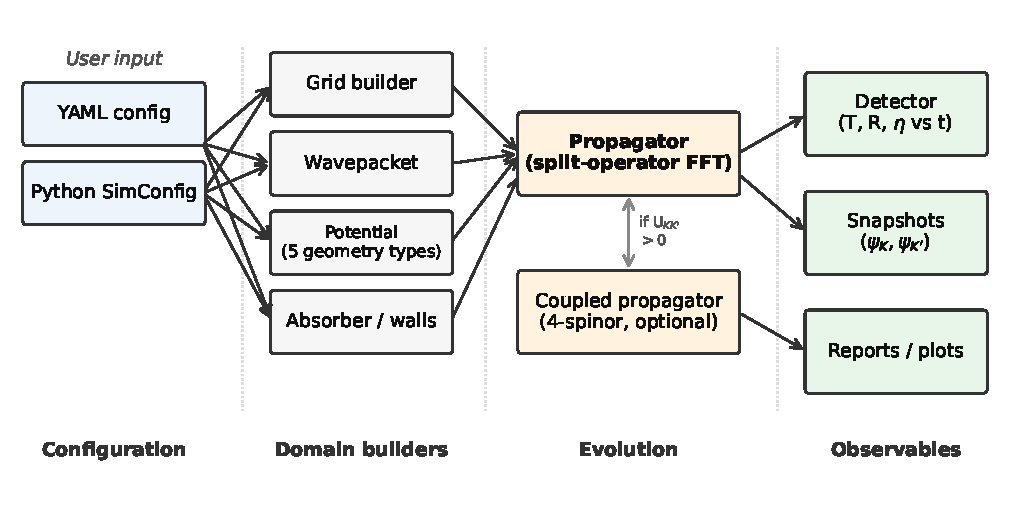
\includegraphics[width=0.82\textwidth]{figs/fig_arch.pdf}
\caption{Architecture of \dirac. Inputs (YAML or Python dataclass)
         flow through grid, wavepacket, and potential builders into
         the propagator; the absorber captures transmitted and
         reflected probability into the detector, which records the
         full transport record. An optional $4$-spinor coupled
         propagator is selected automatically when intervalley
         coupling is enabled.}
\label{fig:arch}
\end{figure*}

\subsection{Software functionalities}

The public API is a small set of top-level imports:
\texttt{SimConfig}, \texttt{load\_config}, \texttt{run\_simulation},
plus the grid, wavepacket, potential, and detector builders. A
typical YAML configuration is loaded and run in three lines:

\begin{verbatim}
from dirac_wavepacket import load_config, run_simulation
cfg = load_config("my_config.yaml")
result = run_simulation(cfg, save_wf=True)
\end{verbatim}

Four features distinguish the package from general-purpose
Schr\"odinger solvers.

\textbf{Tilted and anisotropic dispersions.} The physics
configuration accepts independent Fermi velocities $v_x, v_y$ and a
tilt vector $(w_x, w_y)$ that is reversed automatically at the $K'$
valley by the propagator. Dual-valley runs launch both valleys in
parallel and report the time-resolved valley polarisation
$\eta(t)=(T_K-T_{K'})/(T_K+T_{K'})$.

\textbf{Arbitrary barrier geometry.} The potential builder supports
rectangular, p--n junction, rotated parallelogram, arbitrary
(convex or non-convex) polygonal, and additive multi-barrier
landscapes, with optional sigmoid interface smoothing. Rotated
barriers of any angle are specified by four edge positions and are
the basis of the all-electrostatic valley filter in our first
example.

\textbf{Drain contacts as detectors.} Absorbing drains and channel
walls are implemented consistently with the Dirac structure and their
absorption is bookkept as cumulative $T(t)$, $R(t)$, $P_y(t)$
histories. Auto-stop on small residual probability is enabled by
default and typically shortens runs by $2\text{--}3\times$.

\textbf{Optional intervalley coupling.} A 4-spinor coupled
propagator supports a spatially local, pseudospin-preserving coupling
$U_{KK'}(x,y)\cdot \mathbb{I}_2$; the propagator automatically
reduces to two independent 2-spinor evolutions when the coupling
amplitude is zero. This equivalence is explicitly asserted by the
test suite.

Three console-script sweep drivers (\texttt{dwp-sweep},
\texttt{dwp-sweep-v0}, \texttt{dwp-sweep-vsd}) wrap the
simulation for $V_0$, geometry, and source--drain bias scans with
per-task JSON checkpoints and \texttt{--resume} support.

% =======================================================================
\section{Illustrative examples}
\label{sec:examples}
% =======================================================================

Two self-contained example scripts in the \texttt{examples/}
directory exercise the core capabilities. Both support a
\texttt{--quick} flag for laptop-scale smoke testing and a
publication-quality default mode. Full input parameters are in the
scripts; here we summarise inputs and outputs only.

\subsection{Example 1: all-electrostatic valley filter}

A Gaussian wave packet is launched at normal incidence through a
rectangular barrier ($V_0=1.75\,\EF$) in a channel with transverse
tilt $w_y=0.3\,\vF$. Two runs are compared via a \texttt{--barrier}
flag (Fig.~\ref{fig:ex1}): a straight control barrier at $\alpha=0$
and a rotated filtering barrier at $\alpha=20^\circ$. The results
(Table~\ref{tab:ex1}) are $T_K = T_{K'} = 0.976$, $\eta=0$ for the
control and $T_K=0.716$, $T_{K'}=0.416$, $\eta=+0.265$ for the
filter. The tilt alone does not produce polarisation at a straight
barrier; rotating the same barrier by $20^\circ$ is sufficient to
generate a large valley polarisation by purely electrostatic means.

\begin{table}[h]
\centering
\small
\begin{tabular}{lccc}
\toprule
Barrier & $T_K$ & $T_{K'}$ & $\eta$ \\
\midrule
rect ($\alpha=0$)          & 0.976 & 0.976 & $\phantom{+}0.000$ \\
angled ($\alpha=20^\circ$) & 0.716 & 0.416 & $+0.265$ \\
\bottomrule
\end{tabular}
\caption{Example 1 transmission results; $\eta=(T_K-T_{K'})/(T_K+T_{K'})$.}
\label{tab:ex1}
\end{table}

\begin{figure*}[t]
\centering
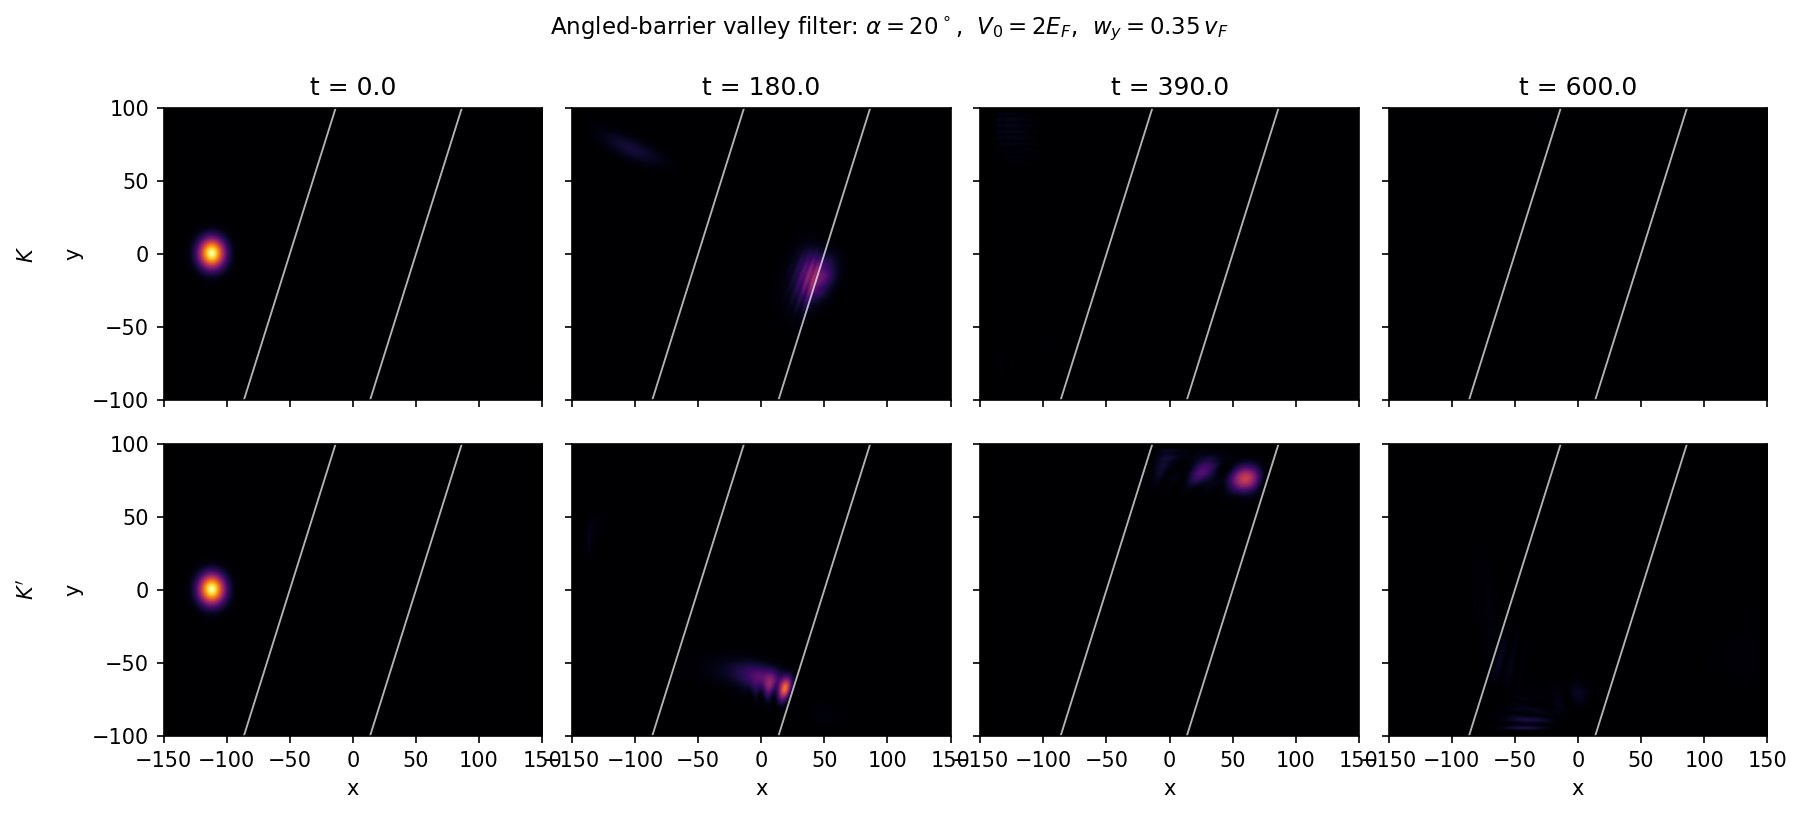
\includegraphics[width=0.92\textwidth]{figs/fig_ex1_angled.png}
\caption{Example 1 (angled barrier, $\alpha=20^\circ$).
         Top row: $K$ wave packet; bottom row: $K'$. Barrier outlines
         in blue, drain regions shaded. $K$ transmits cleanly to the
         right drain while $K'$ is reflected back, yielding
         $\eta=+0.265$.}
\label{fig:ex1}
\end{figure*}

\subsection{Example 2: angular dependence of Klein tunneling}

The second example exercises the untilted, isotropic Dirac limit. A
rectangular barrier at $V_0=2\,\EF$ is probed by a single-valley
wave packet at a list of injection angles; at zero tilt $K$ and $K'$
are equivalent. Four angles $\{-15^\circ, -5^\circ, +5^\circ,
+15^\circ\}$ are scanned in a single invocation
(Fig.~\ref{fig:ex2}). The transmission peaks near $\theta=0$ (the
Klein paradox), and drops off with $|\theta|$;
$T(\pm5^\circ)=0.974$, $T(\pm15^\circ)=0.868$. The mirror-symmetry
residuals between $\pm\theta$ pairs are
$|\Delta T| \sim 10^{-6}$, confirming the propagator's numerical
symmetry at single precision.

\begin{figure*}[t]
\centering
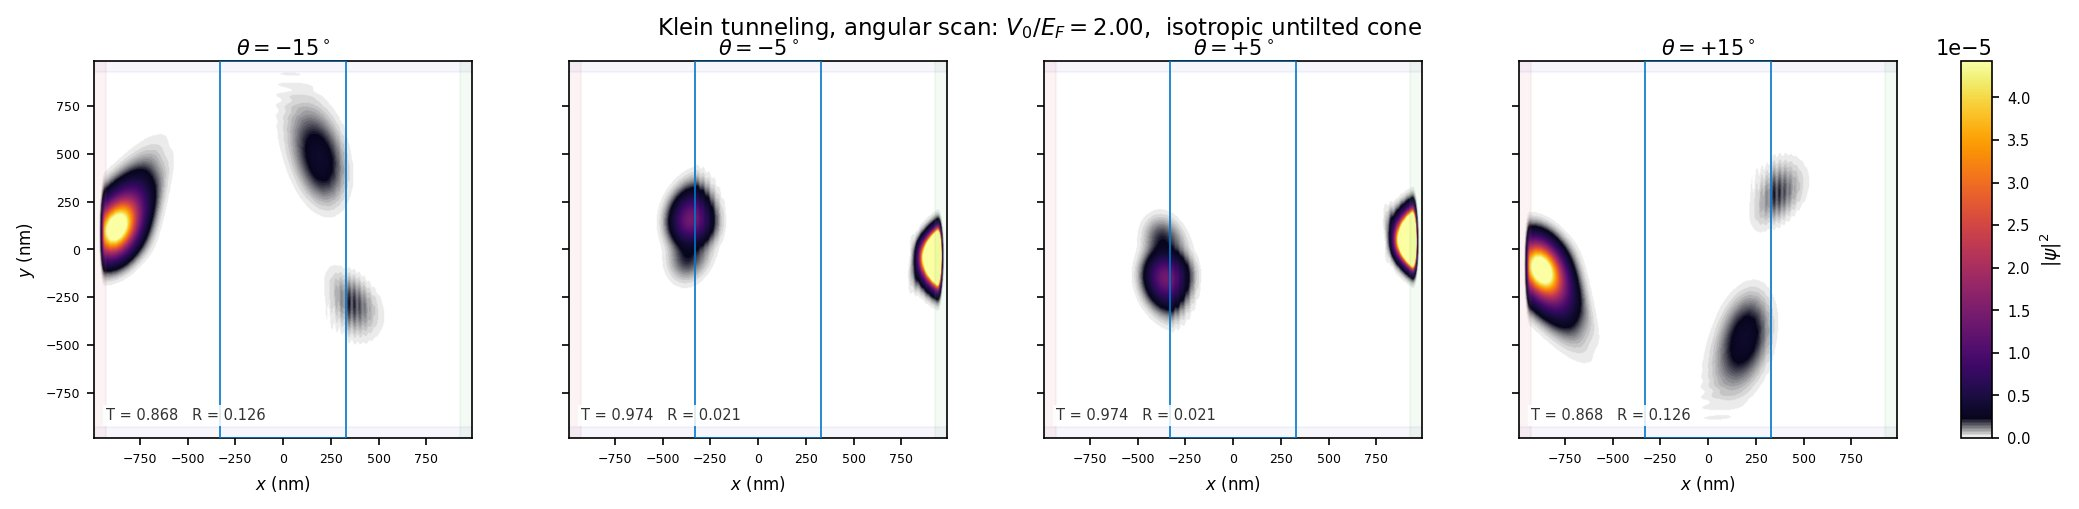
\includegraphics[width=0.92\textwidth]{figs/fig_ex2_snapshots.png}
\caption{Example 2 Klein-tunnelling angular scan. Four single-valley
         runs at $\theta \in \{-15^\circ, -5^\circ, +5^\circ,
         +15^\circ\}$ through a rectangular barrier of height
         $V_0=2\,\EF$. Mirror-symmetric pairs
         ($\theta \leftrightarrow -\theta$) are numerically
         coincident to $|\Delta T| \sim 10^{-6}$.}
\label{fig:ex2}
\end{figure*}

\begin{figure}[h]
\centering
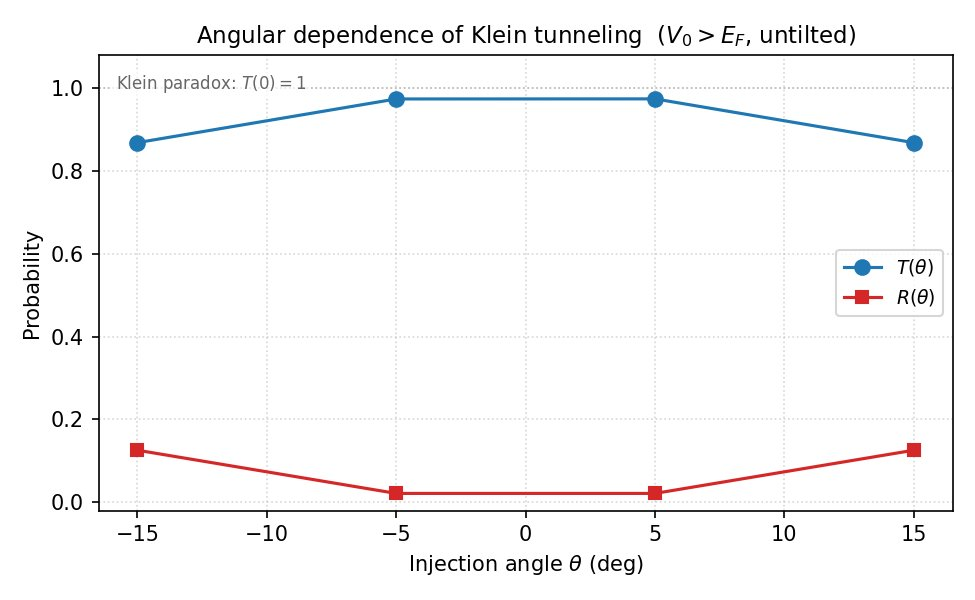
\includegraphics[width=\linewidth]{figs/fig_ex2_summary.png}
\caption{Summary of Example 2: $T(\theta)$ (blue) approaches the
         Klein-paradox limit $T=1$ near $\theta=0$ and decreases
         with $|\theta|$; $R(\theta)$ (red) is the complement.}
\label{fig:ex2sum}
\end{figure}

A pytest suite (eight tests, ${\sim}40\,\mathrm{s}$ total) asserts
norm conservation, mirror symmetry, coupled--independent equivalence
at zero intervalley coupling, polygon / shaped barrier equivalence,
and Klein-paradox agreement with the analytical
Katsnelson transfer-matrix formula~\cite{Katsnelson2006}.

% =======================================================================
\section{Impact}
\label{sec:impact}
% =======================================================================

\dirac enables new research questions at the intersection of Dirac /
Weyl electron optics and realistic device modelling. Our group has
used the package as the computational engine for a study of
all-electrostatic valley phase gates in tilted Dirac
channels~\cite{Yesilyurt2026phasegate}. Example~1 of the present
paper also reproduces, via time-dependent wave-packet simulation,
the all-electrostatic valley-filtering effect originally obtained in
Ref.~\cite{Yesilyurt2026valleyfilter} by wave-function matching
(transfer matrix) and semiclassical ray tracing, providing
independent numerical confirmation of that result. The package
enables systematic parameter scans (barrier geometry, tilt magnitude
and direction, intervalley coupling amplitude, source--drain bias)
that are impractical with tight-binding scattering-matrix codes on
realistic device sizes, and it resolves time-dependent information
(transient $\eta(t)$, wave-packet trajectories, Fabry--Pérot
build-up) that is inaccessible to stationary methods.

Beyond our own use, \dirac is intended as an installable tool for
the broader 2D-materials device community. The installation is
\texttt{pip install dirac-wavepacket} from the archived source; no compilation
is required, no GPU is mandatory, and a typical production run
completes in 10--30 minutes on a standard workstation. The YAML
configuration interface means users can reproduce published
simulations by sharing a config file rather than a full code diff.
The pytest suite and auto-grid validator give new users a fast way
to check that a chosen grid / time step combination is numerically
sound before launching long runs. Compared with the
continuum-Schr\"odinger neighbours \textsc{pytalises}
\cite{pytalises} and \textsc{qmsolve} \cite{qmsolve} the package
occupies a distinct physical regime: the Dirac structure,
anisotropic / tilted dispersion, valley chirality, and
Klein-regime-compatible boundaries are not available in the
Schr\"odinger family of solvers.

% =======================================================================
\section{Conclusions}
\label{sec:conclusions}
% =======================================================================

We have presented \dirac, a compact and installable Python package
for time-dependent transport of wave packets in 2D Dirac and Weyl
systems with tilted, anisotropic cones. The core is a second-order
split-operator Fourier propagator with an analytical $2\times2$
momentum-space unitary and a validated optional $4$-component
coupled extension. Arbitrary polygonal or rotated barriers,
drain-as-detector bookkeeping, and mass-wall confinement are
supported out of the box. Two worked examples demonstrate the
key capabilities and the test suite locks them down with tight
physical invariants. Planned extensions include GPU acceleration via
CuPy and a companion package for valley-resolved phase extraction
from saved wavefunction snapshots.

\section*{Acknowledgements}
The author thanks the Nanoelectronics Research Center for computing
resources.

\begin{thebibliography}{00}

\bibitem{CastroNeto2009}
A.\,H. Castro Neto, F. Guinea, N.\,M.\,R. Peres, K.\,S. Novoselov,
A.\,K. Geim, The electronic properties of graphene, Rev.\ Mod.\
Phys.\ 81 (2009) 109--162.

\bibitem{Goerbig2008}
M.\,O. Goerbig, J.-N. Fuchs, G. Montambaux, F. Pi\'echon, Tilted
anisotropic Dirac cones in quinoid-type graphene and
$\alpha$-(BEDT-TTF)$_2$I$_3$, Phys.\ Rev.\ B 78 (2008) 045415.

\bibitem{Nguyen2018}
V.\,H. Nguyen, J.-C. Charlier, Klein tunneling and electron optics
in Dirac--Weyl fermion systems with tilted energy dispersion, Phys.\
Rev.\ B 97 (2018) 235113.

\bibitem{Zhang2018}
S.-H. Zhang, W. Yang, Oblique Klein tunneling in 8-Pmmn borophene
p--n junctions, Phys.\ Rev.\ B 97 (2018) 235440.

\bibitem{LopezBezanilla2016}
A. Lopez-Bezanilla, P.\,B. Littlewood, Electronic properties of
8-Pmmn borophene, Phys.\ Rev.\ B 93 (2016) 241405(R).

\bibitem{Zabolotskiy2016}
A.\,D. Zabolotskiy, Yu.\,E. Lozovik, Strain-induced pseudomagnetic
field in the Dirac semimetal borophene, Phys.\ Rev.\ B 94 (2016)
165403.

\bibitem{Soluyanov2015}
A.\,A. Soluyanov et al., Type-II Weyl semimetals, Nature 527 (2015)
495--498.

\bibitem{Wang2019}
Q. Wang, C. Yesilyurt et al., Room-temperature nonlinear Hall effect
and wireless radio-frequency rectification in Weyl semimetal
T$_d$-MoTe$_2$, Nano Lett.\ 19 (2019) 2647--2653.

\bibitem{Berry1987}
M.\,V. Berry, R.\,J. Mondragon, Neutrino billiards: Time-reversal
symmetry-breaking without magnetic fields, Proc.\ R.\ Soc.\ Lond.\ A
412 (1987) 53--74.

\bibitem{Katsnelson2006}
M.\,I. Katsnelson, K.\,S. Novoselov, A.\,K. Geim, Chiral tunnelling
and the Klein paradox in graphene, Nat.\ Phys.\ 2 (2006) 620--625.

\bibitem{Groth2014}
C.\,W. Groth, M. Wimmer, A.\,R. Akhmerov, X. Waintal, Kwant: a
software package for quantum transport, New J.\ Phys.\ 16 (2014)
063065.

\bibitem{Kloss2021}
T. Kloss, J. Weston, B. Gaury, B. Rossignol, C. Groth, X. Waintal,
Tkwant: a software package for time-dependent quantum transport,
New J.\ Phys.\ 23 (2021) 023025.

\bibitem{Mocken2008}
G.\,R. Mocken, C.\,H. Keitel, FFT-split-operator code for solving
the Dirac equation in 2+1 dimensions, Comput.\ Phys.\ Commun.\ 178
(2008) 868--882.

\bibitem{pytalises}
S. Vowe, pytalises: an easy-to-use Python implementation of the
split-step Fourier method for the time-dependent Schr\"odinger
equation (2020). \url{https://github.com/savowe/pytalises}.

\bibitem{qmsolve}
quantum-visualizations, qmsolve: a module for solving and
visualising the Schr\"odinger equation (2022).
\url{https://github.com/quantum-visualizations/qmsolve}.

\bibitem{Yesilyurt2026valleyfilter}
C. Yesilyurt, All-electrostatic valley filtering by barrier rotation
in tilted Dirac channels, arXiv:2603.03117 (2026).
\url{https://doi.org/10.48550/arXiv.2603.03117}.

\bibitem{Yesilyurt2026phasegate}
C. Yesilyurt, All-electrostatic valley phase gates in tilted Dirac
channels, arXiv:2603.11635 (2026).
\url{https://doi.org/10.48550/arXiv.2603.11635}.

\end{thebibliography}

\section*{Current executable software version}
\label{}

\begin{table}[!h]
\small
\begin{tabular}{|c|p{4.8cm}|p{6.8cm}|}
\hline
\textbf{Nr.} & \textbf{(Executable) software metadata description} &
              \textbf{Value} \\
\hline
S1 & Current software version & v1.0.0 \\
\hline
S2 & Permanent link to executables of this version &
    \nolinkurl{github.com/can-yesilyurt/Dirac-Wavepacket/releases/tag/v1.0.0} \\
\hline
S3 & Legal Software License & MIT \\
\hline
S4 & Computing platforms / Operating Systems &
    Linux, macOS, Windows (any platform supporting CPython $\geq 3.11$). \\
\hline
S5 & Installation requirements \& dependencies &
    Python $\geq 3.11$; NumPy, SciPy, Matplotlib, PyYAML;
    optional pyFFTW. Install via \texttt{pip install -e .}
    from the cloned repository. \\
\hline
S6 & If available, link to user manual &
    \nolinkurl{github.com/can-yesilyurt/Dirac-Wavepacket/tree/main/docs} \\
\hline
S7 & Support email for questions & \texttt{cyesil@nanorescenter.com} \\
\hline
\end{tabular}
\caption{Executable software metadata (mandatory).}
\label{tab:meta-exe}
\end{table}

\end{document}
